\section{RESULT AND DISCUSSION}
In line with the methodology used above, this project was tested in Gazebo Classic and RViz2 based on ROS2 Humble. The first is a replication of the problem to be solved in this project. Two obstacles that are prominent to this problem were added to the simulated world to be tested separately:
1. Bookshelf: Due to the thin partitions on each level of the bookshelf, the LiDAR scanning surface that is not at the same level as one of the shelf will not detect the shelf, but only the baffles on either side. To visualise this more, the back plate of the shelf was removed and the shelf was then placed directly in front of the robot and mapped using only LiDAR. At this point it can be seen in RViz2 that only the baffles appear as obstacles in the generated map. If the robot is given a forward navigation command in this case, it will move straight ahead and hit the bookshelf. It will not be able to navigate correctly and at the same time it will destroy the original map as shown in the figure.
\begin{figure}[H]
    \centering
    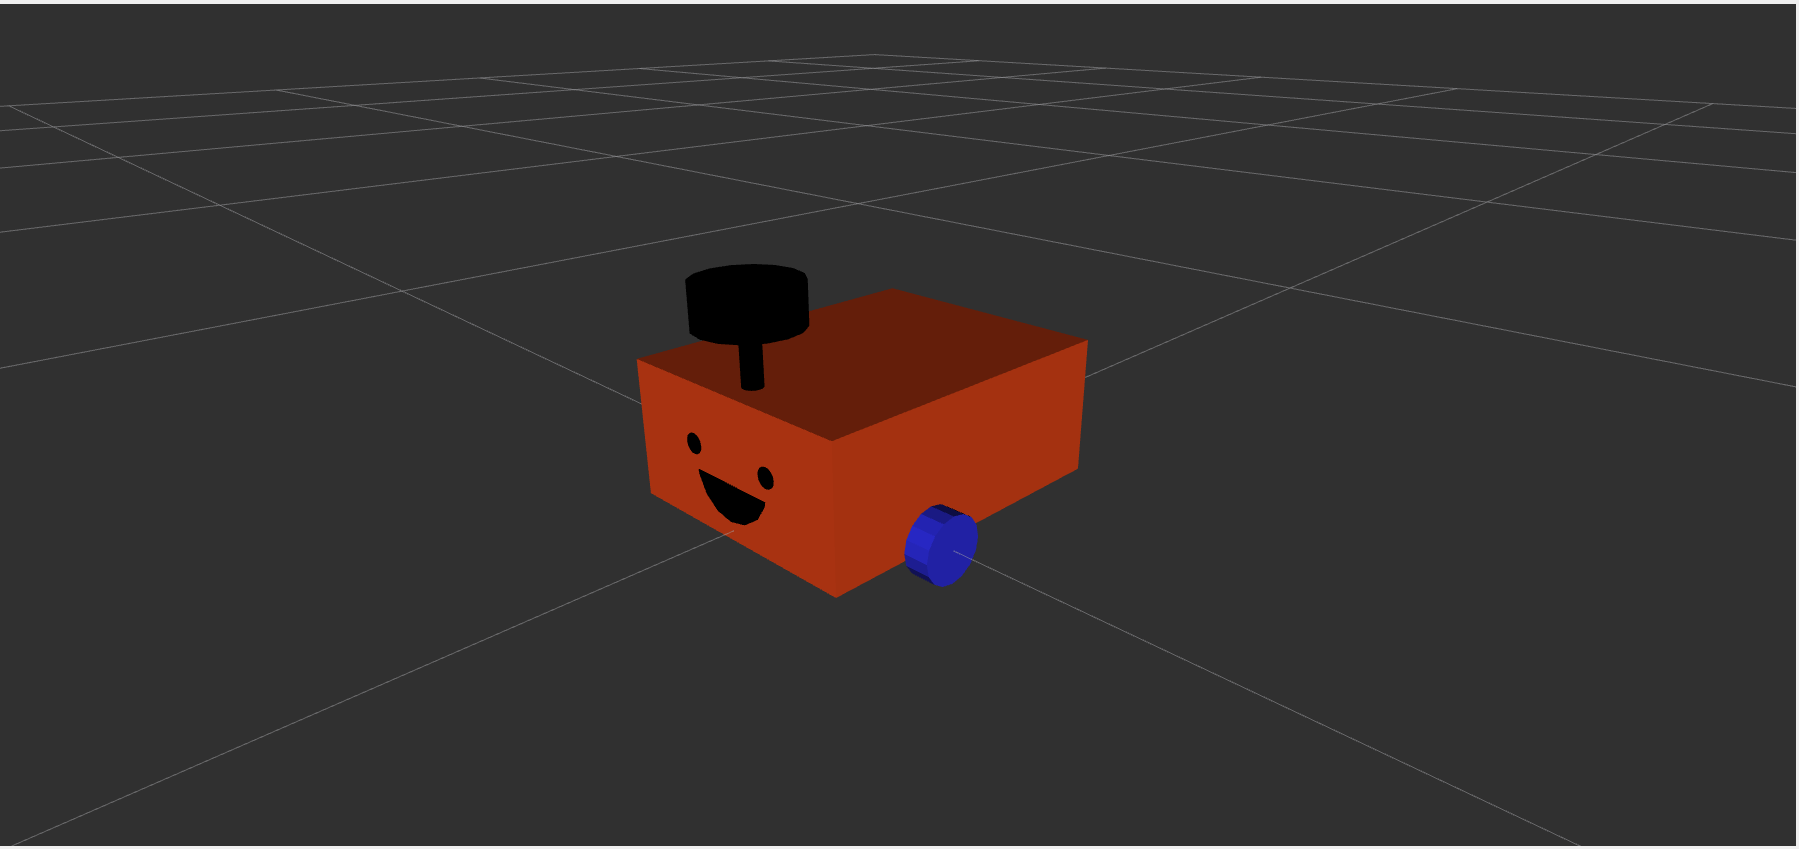
\includegraphics[width=0.8\linewidth]{figs/robot.png}
    \caption{Example figure caption.}
\end{figure}
After using the merged LaserScan data returned by the fusion algorithm, it is clear in RViz2 that the baseboard of the bookshelf was successfully recognised as an obstacle and mapped.
\begin{figure}[H]
    \centering
    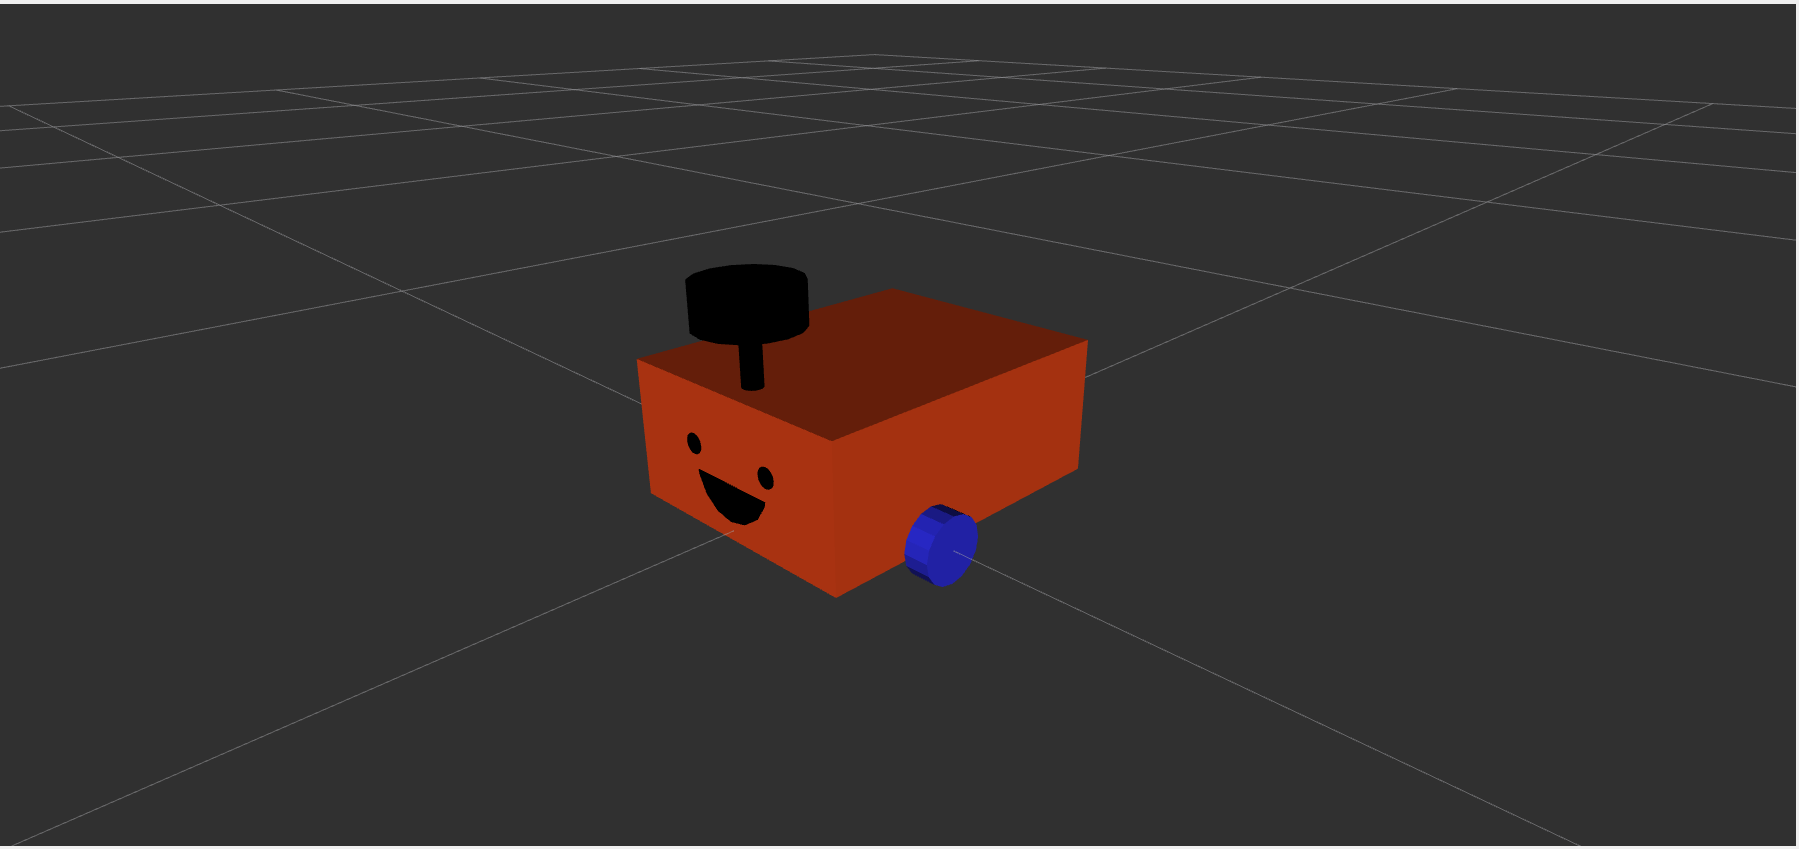
\includegraphics[width=0.8\linewidth]{figs/robot.png}
    \caption{Example figure caption.}
\end{figure}
2. Barricades: Another very intuitive test is this cylinder barricade with a polygonal bottom cross-section and a rounded upper cross-section. As shown in the figure.
\begin{figure}[H]
    \centering
    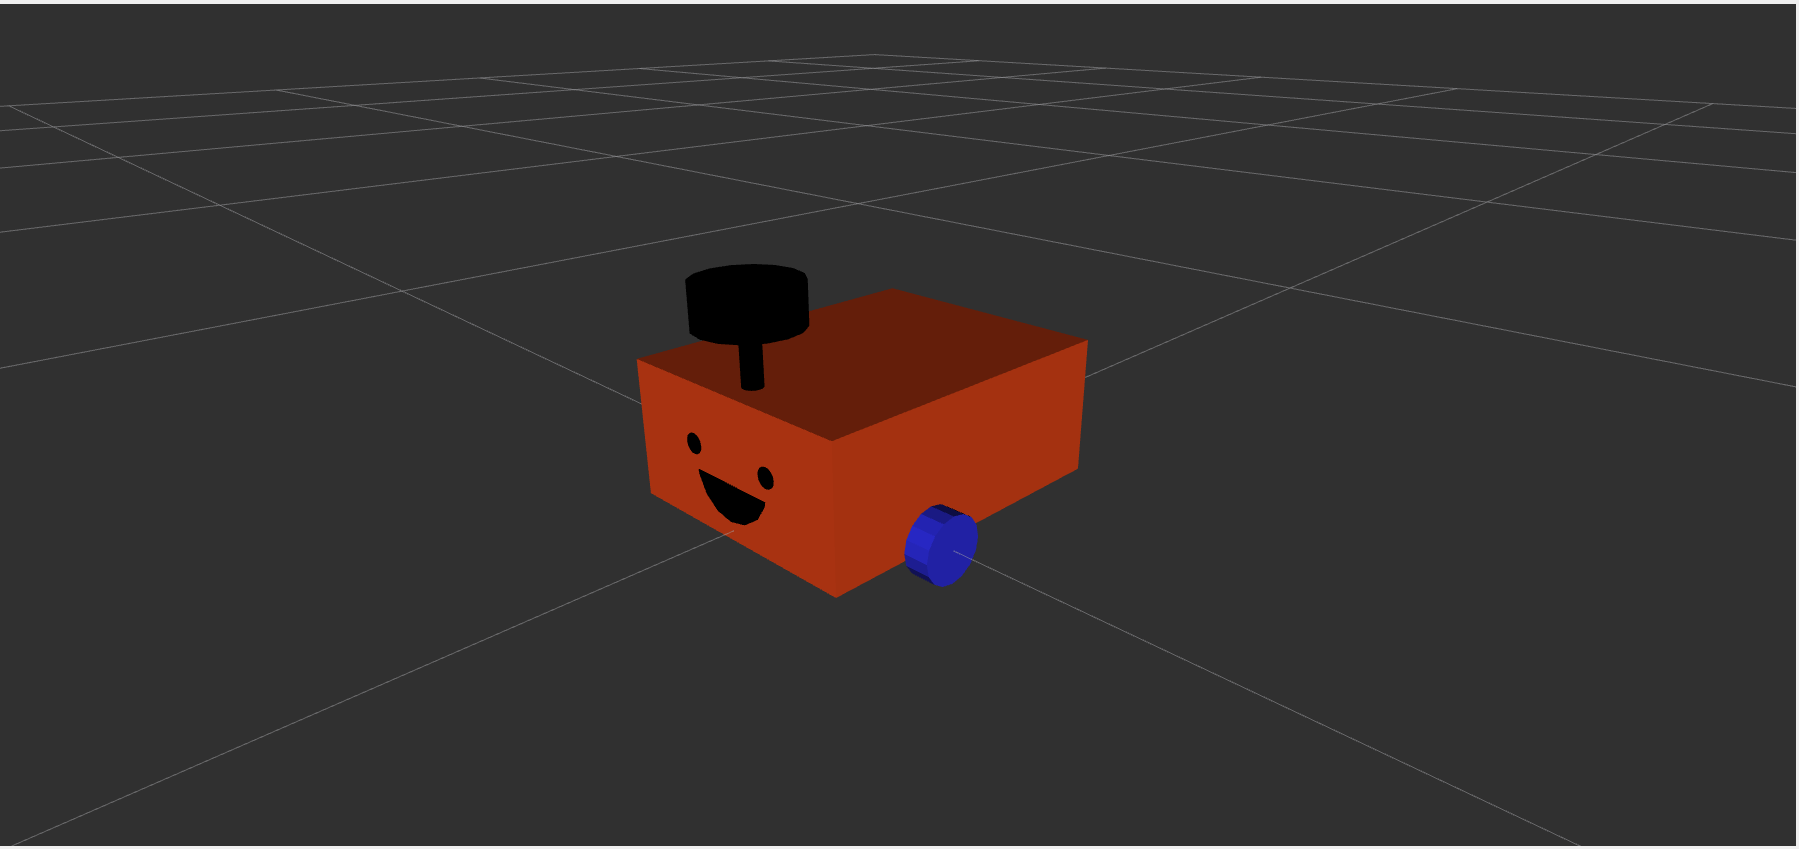
\includegraphics[width=0.8\linewidth]{figs/robot.png}
    \caption{Example figure caption.}
\end{figure}
The different shapes of such barricades at different heights make it very straightforward to see whether low-lying obstacles are detected or not, even without the need to build a map. Both the LiDAR LaserScan data and the merged LaserScan data returned by the fusion algorithm, distinguished by different colours, are turned on in RViz2:
\begin{figure}[H]
    \centering
    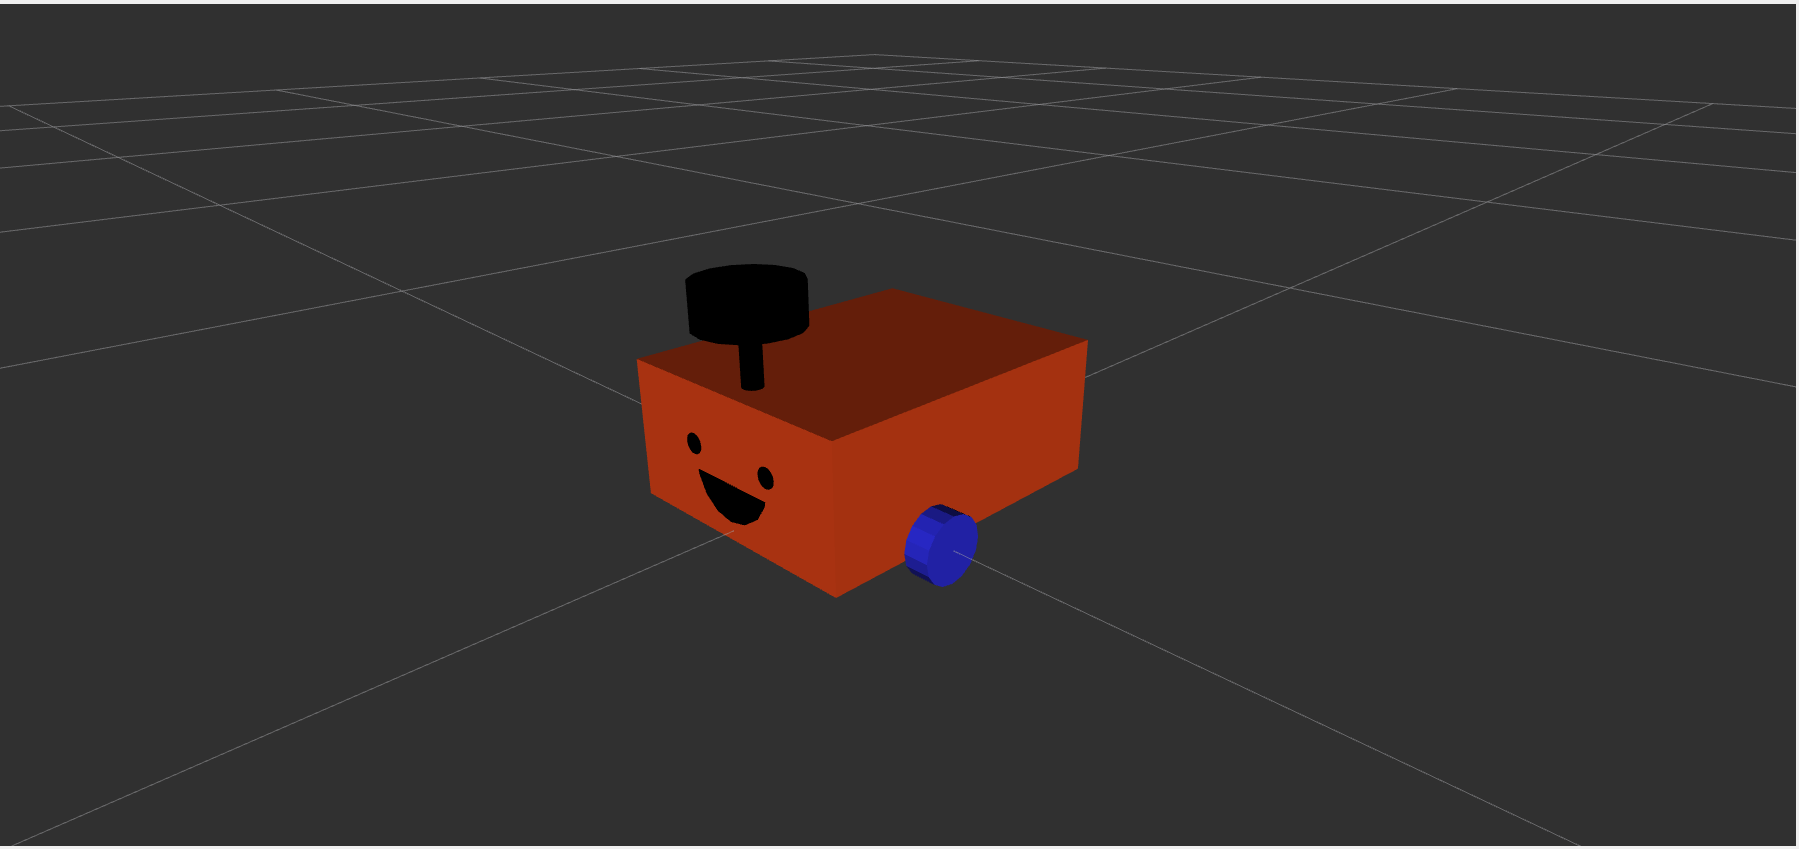
\includegraphics[width=0.8\linewidth]{figs/robot.png}
    \caption{Example figure caption.}
\end{figure}
It can be seen that what was scanned before the fusion was the higher part of the top half with a circular cross-section, whereas after the merger the scanning of this area was replaced with the lower part of the bottom cross-section with a polygonal shape. This also represents the fulfilment of the objectives of this project.




